\chapter{Introduction}
\label{chapter:intro}
\setlength{\epigraphwidth}{3in}
\epigraph{A picture is worth a thousand words.\\[1mm] But how many can the machine
say?}

The famous English adage states "A picture is worth a thousand
words"~\cite{ThousandQuote}. This is meant to convey that there is a lot the
viewer can learn/infer from a single still image and enumerating all the
information encoded in an image can use up even a thousand words. This is
illustrated in our extensive use of images in all forms of communication, from
scientific journals to Twitter chats. 
%
Humans are very good at processing images and videos and gathering all this
encoed information, but the computers still struggle to maks sense of the
simplest ones.
%
One could even say it is still easier for computers to store, parse, search and
even understand a thousand words than a single image.
%
The usage of multimedia on the internet has grown to staggering levels in the
last few yeas, due to easy access to cameras through smart phones. For eg. about
95 million photos are uploaded to Instagram every day~\cite{InstStats} and about
400 hours of video is uploaded to Youtube every minute~\cite{YouStats}. This
presents both an enoromous challenge and an oppurtunity to build smarter
computer algorithms to summarize and understand this data. Such algorithms could
hlep us index and search this huge amount of data better. \fixme{Something
something about general AI}.
%

One such problem at the heart of machine understanding of visual media, is
automatic captioning of images and videos. This involves designing an algoritm
which takes the image or the video as input and generates a natural language
caption describing succintly the content of the media. Effectively solving this
problem requires the machine to be able to identify the salient objects in the
image/video, their states and the relationship between these objects and also
correctly recognize the scene. It needs to be able to use this information to
generate a natural language caption summarizing it.

%%TODO: SHOULD THIS GO to literature review of features?
Until recently, the task of identifying even a single object in an image
reliably on a large datasets was hard. This changed dramatically with the
availaibility of large scale annotated data like the ImageNet
dataset~\cite{ImagenetOrig}, and  application of deep learning techniques,
specifically convolutional neural networks (CNN). For example, in the image
classification task of the ImageNet Large Scale Visual Recognition
Challenge~\cite{ILSVRC15} (ILSVRC), which involves classifying images to one of
thousand object classes, the accuracy has improved from 71.8\% to 95.06\%,
surpassing the human performance on the same task. 

It was also discovered that object classification networks which are trained on
the large imagenet dataset, also generalize very well and can used as generic
image feature extraction for different tasks~\cite{yosinski2014transferable}.
This has led to successful application of such deep networks to various other
tasks in computer vision including the task of image captioning XXX: some
citations.

In this thesis we will examine the task of automatic image/video captioning and
discuss algorithms based on deep learning to solve this task. We will discuss
the relavant literature, ....................................

%XXX: Talk about recent interest and mention the two stage pipeline with
%references. 

\begin{figure}[h]
	\centering
	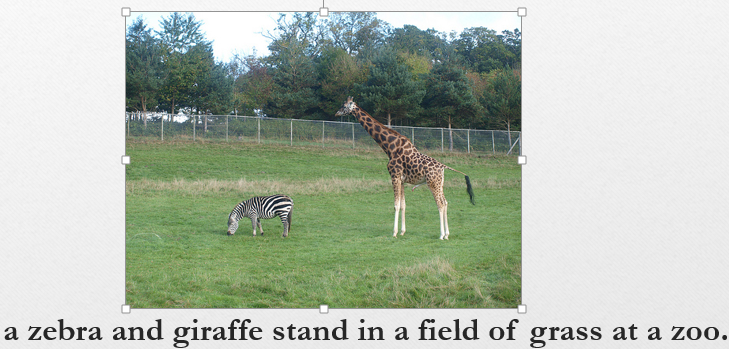
\includegraphics[width=0.9\textwidth]{./images/ExampleCaption.png}
	\caption{A sample image caption pair from the MS-COCO dataset}
	\label{fig:ExampleCap}
\end{figure}


Outlining the computer vision problem of labelling objects, how advent of CNN
has almost solved single object identification and to an extent multiple object
id and localization. With references ofcourse

More challenging problem is generating descriptive lables i.e captions
A precursor to the generic problem of machines understanding visual media. 

\fixme{(Piece together from the report and the ACMMM paper, about 1 page)}

\section{Problem Statement}

Our task is to generate a caption given an input image or video. We are going to
focus on methods to generate a single sentence caption only. Thus a caption can
be precisely defined to be a sentence, $S$, which is a sequence of words $(w_0,
w_1,\cdots, w_{n-1})$ with $n$ being the length of the sentence. Thus we are
trying to learn the distribution, $P(S|V)$, where V is the visual input (either
an image or a video). This can be written as in eq.\ref{eq:langB1}. 

\begin{equation}
\label{eq:langB1} P(S|V) = P(w_0 w_1 \cdots w_{n-1}|V)
\end{equation}

We will take a two staged approach to model this probability distribution, as
has been popular in the image captioning literature. In the first stage the
visual input $V$ is mapped onto one or more feature vectors $V_f$. This process
is deterministic and the feature vectors extracted are of fixed size for every
input. In this thesis, we will explore different methods for extracting feature
vectors from images and videos and analyze their performance quantitatively and
qualitatively on the automatic captioning task. 

For images, we will experiment with features extracted from CNNs trained on
ImageNet for single object classification, binary object detector features, and
features constructed from object localization networks \fixme{XXX: references}.
In case of videos, we will explore dense trajectory features, frame-level
feature extraction and 3D convolutional features. 

Next stage, is the languge model, which takes the visual feature vector $V_f$ as
input and learns a probability distibution over sentences. Since the sentences
are sequence of words, they lend themselves naturally to be modelled using
sequential models like recurrent neural networks. In this thesis we will only
deal with language models based on the recurrent networks. We will implement and
analyze a popular implementation proposed in literature. Then we explore some
extensions like using deeper networks with residual connections, class based
factorization of the language model and also experiment with a model based on
bi-directional recurrent networks. We will also discuss several techniques to
create an ensemble of language models, exploring the non-trivial problem of
picking one best caption from a pool of arbitrary length captions from each
model in the ensemble.

Evaluating an image captioning system is also non-trivial, since we have to
compare the generated caption against a few different references captions. The
standard \fixme{recipe} followed in the literature, which we also uses here, is
to use multiple automatic evaluation metrics adopted from machine translation
field. In addition, we also present human evaluation results obtained from our
participation in three automatic captioning challenges. Concretely, we
participated in the Microsoft COCO Image Captioning Challenge 2015, Large Scale
Movie Description Challenge 2015 and the Microsoft Video to Text Challenge 2016
and we will present the results and the \fixme{knowledge} gained from these.
\fixme{XXX: references}.

We analyze the results of the experiments qualitatively and discuss strengths
and shortcomings of current solutions. Drawing from this analysis, we discuss a
few promising new directions the research on vision and language is heading.

In summary, the main contributions of this thesis are as follows:
    - Basic Image captioning pipeline in detail
    - Then take apart each block and see how we can improve it
    - Then measure and demonstrate if these actually help
    - In depth analysis of  what are the strengths and weaknesses of current
    approaches
    - Put forth several ideas for what we could do next.

\begin{itemize}
    % You can use this command to set the items in the list closer to each other
    % (ITEM SEParation, the vertical space between the list items) 
    \setlength{\itemsep}{0pt}
    \item Nelli Portal (Aalto Library): \url{http://www.nelliportaali.fi}
    \item ACM Digital library: \url{http://portal.acm.org/}
    \item IEEExplore: \url{http://ieeexplore.ieee.org}
    \item ScienceDirect: \url{http://www.sciencedirect.com/}
    \item \ldots although Google Scholar (\url{http://scholar.google.com/}) will
    find links to most of the articles from the abovementioned sources, if you
    search from within the university network
\end{itemize}

\fixme{Write Fresh 1-1.5 pages}

\section{Structure of the Thesis}
\label{section:structure} 
Describe thesis structure
\fixme{Write Fresh .5 pages}
